\chapter{Introduction}
\pagenumbering{arabic}\hspace{3mm}

Image processing libraries these days (eg. Open CV) uses the conventional methods which have the possibility to be outperformed by methods which leverage the power of artificial intelligence. Some recent research have shown that some of these AI based methods are able to perform atleast as good as conventional approaches. The aim of this project is to implement, apply and possibly improve upon the existing approaches in Digital Image Processing and Computer Vision. These common tasks can include (not limited to) applications like: Image Compression, Denoising, Super Resolution, Flow Estimation, Object Detection, etc.


\section{Image Processing}

\begin{figure}[!ht]
    \centering
    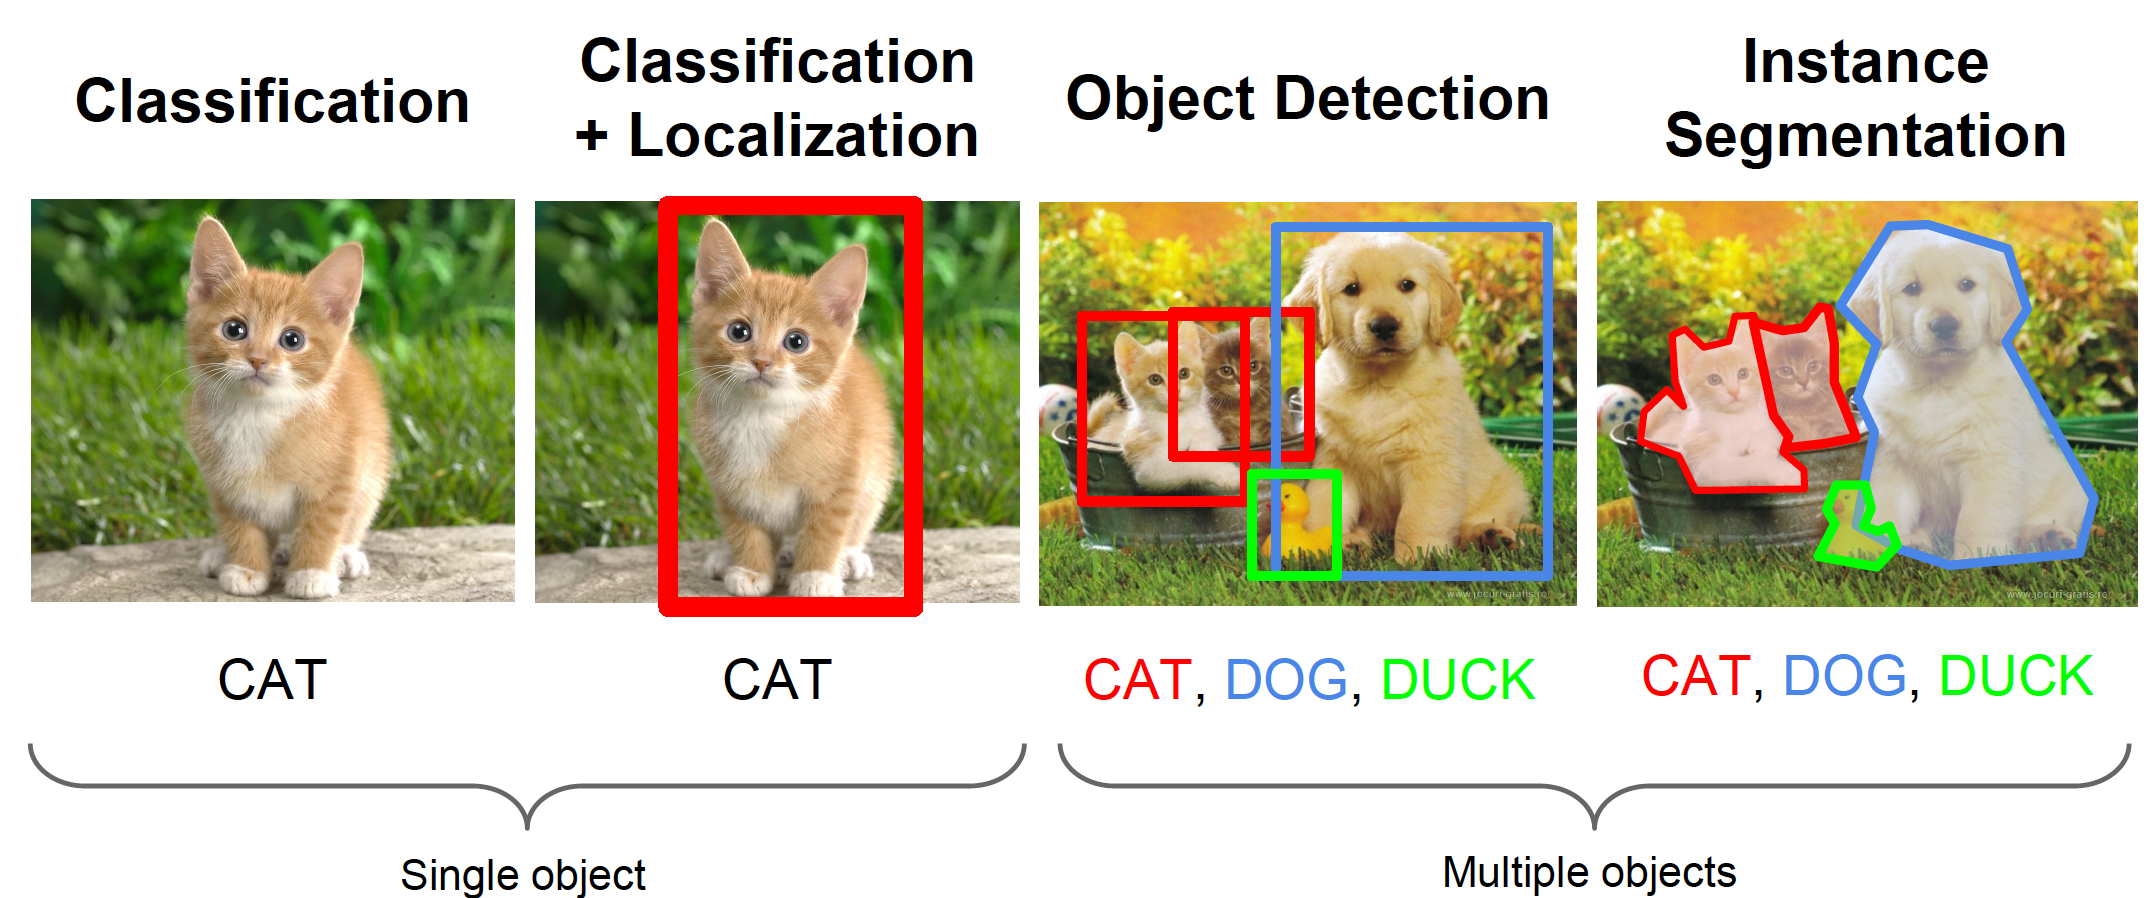
\includegraphics[width=0.75\textwidth]{fig/1-1.png}
    \captionsource{Examples of pattern recognition}
    {\href{https://www.cs.cornell.edu/courses/cs4670/2016sp/lectures/lec41_recowrapup_web.pdf}{www.cs.cornell.edu}}
    \label{fig:exPatternRecognition}
\end{figure}

Image processing is manipulating an image in order to enhance it or extract information from it. It is widely useed in medical visualization, biometrics, self-driving vehicles, gaming, surveillance, and law enforcement. It can used in various ways: visualization, restoration, imformation retrieval, pattern recognition, etc.

General approach of image processing involves eight key phases: image acquisition, image enhancement, image restoration, color space transformation, compression or decompression, morphological processing, recognition, and representation. It is very difficult to carry out these steps manually on a very big data, this is where AI and ML algorithms become very helpful.

\begin{figure}[!ht]
    \centering
    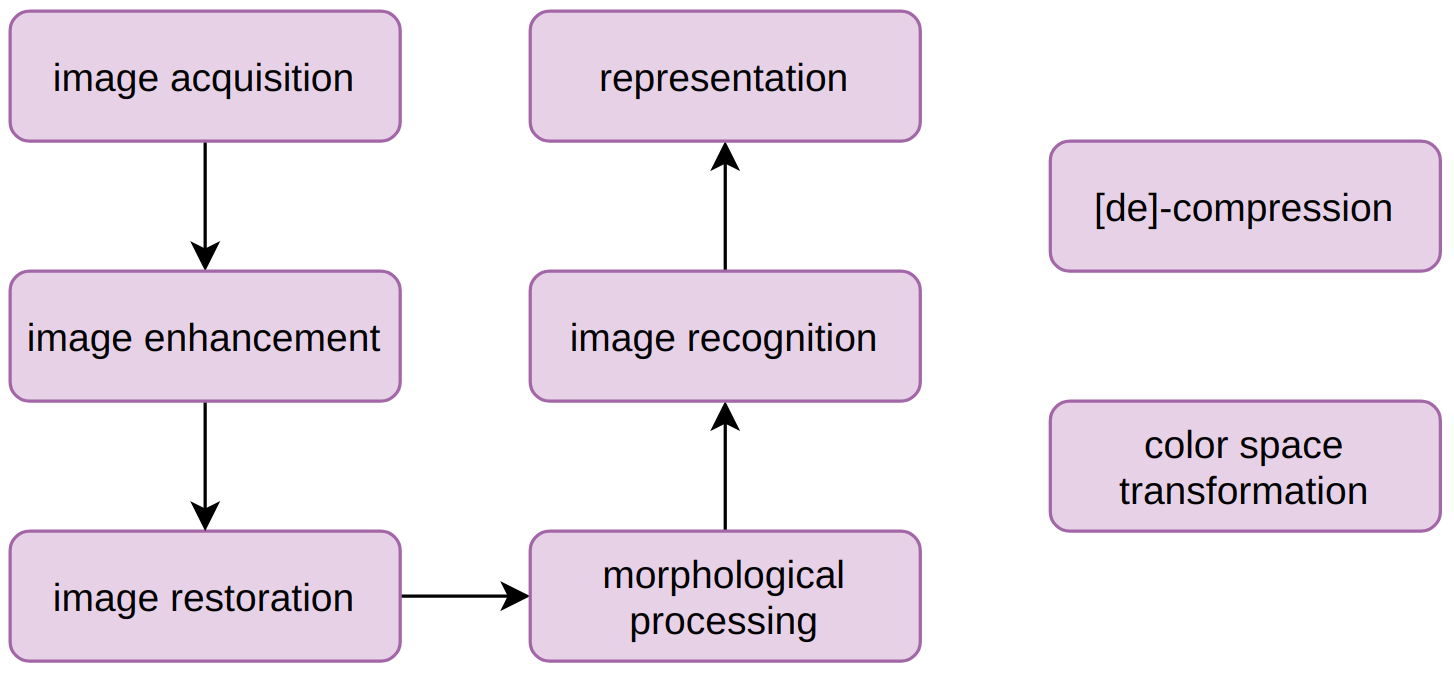
\includegraphics[width=0.75\textwidth]{fig/1-2.png}
    \caption{Key phases of image processing}
    \label{fig:keyPhasesOfImageProcessing}
\end{figure}

\section{Recent advances}

Modern AI algorithms have enabled computer to perform detection, segmentation, recognition, compression, extraction, generation, and discrimination. Every year a state of the art model is invented to solve the existing problem in a better way. It is now an established fact that machines are now better than humans in counting, classifying and segmenting instances. 
